\documentclass{book}[12pt, a4paper, twoside] % Tipo de documento y tamaño de letra.

%%%%%%%%% Preambulo %%%%%%%%%%%%%%%%

% Para modificar los margenes. 
\usepackage{geometry}
\geometry{
    a4paper,
    left=20mm,
    top=20mm,
    right=20mm,
    bottom=20mm,
}

\usepackage[T1]{fontenc}
\usepackage{tocloft}
\usepackage{titlesec}
\setlength{\parskip}{1em} % Ajusta el valor según tus necesidades

\titleformat{\section}[hang]{\normalfont\bfseries}{\thesection}{0.5em}{}
\titleformat{\subsection}[hang]{\normalfont\bfseries}{\thesubsection}{0.5em}{}
\titleformat{\subsubsection}[hang]{\normalfont\bfseries}{\thesubsubsection}{0.5em}{}



% Para la bibliografia.
\usepackage[square,numbers]{natbib}
\usepackage{bibentry}
\nobibliography*

% Recursos personales.

\newcommand\asignatura{
Minería de Datos
}

\newcommand\nombrepec{
\vspace{0.25cm}
Proyecto de minería de datos

}

\newcommand\numeropec{
2
}

% \newcommand{\pec}{PEC}
\newcommand{\PRA}{PRA}

\newcommand\autor{
Álvaro Monforte Marín
}

\newcommand\tipopuntuacion{
% \%
% points
% puntos
p
}



%%%%%%%%%%%%%%%%%%%%%%%%%%%%%%%%%%%%%%%%%%%%%%%%%%%%%%%%%%%%%%%%%%%%%%%%%%%%%%%
% Funciones propias:
%%%%%%%%%%%%%%%%%%%%%%%%%%%%%%%%%%%%%%%%%%%%%%%%%%%%%%%%%%%%%%%%%%%%%%%%%%%%%%%

% Para realizar ejercicios
\newcommand{\ejercicio}[3]{
\ifthenelse{\equal{#1}{true}}{\newpage}{}
\section{Ejercicio #2 \normalsize \textbf{$[#3 \tipopuntuacion]$}}
}

% % Para realizar practicas
% \newcommand{\tematica}[4]{
% \ifthenelse{\equal{#1}{true}}{\newpage}{}
% \section{#2 \textbf{$[#3 \text{\tipopuntuacion}]$}}
% \textbf{#4}
% \vspace{0.15cm}
% % \subsubsection{Respuesta/as al #2}
% }

% \newcommand{\subtematica}[4]{
% \ifthenelse{\equal{#1}{true}}{\newpage}{}
% \subsection{#2 \textbf{$[#3 \text{\tipopuntuacion}]$}}
% \textbf{#4}
% \vspace{0.15cm}
% % \subsubsection{Respuesta/as al #2}
% }


% Para introducir imagenes
% (ejemplo: \insertimage{nombre_de_la_imagen}{ancho_de_la_imagen}{leyenda_de_la_imagen})

\usepackage{graphicx}
\usepackage{float}

\newcommand{\imagen}[3]{
\begin{figure}[H]
\centering
\includegraphics[scale=#2]{#1}
\caption[#3]{#3}
\label{fig:#1}
\end{figure}
}


%%%%%%%%%%%%%%%%%%%%%%%%%%%%%%%%%%%%%%%%%%%%%%%%%%%%%%%%%%%%%%%%%%%%%%%%%%%%%%%%%%%%%%
\newcommand{\documento}[2]{\href{#1}{#2}}
%%%%%%%%%%%%%%%%%%%%%%%%%%%%%%%%%%%%%%%%%%%%%%%%%%%%%%%%%%%%%%%%%%%%%%%%%%%%%%%%%%%%%%


%%%%%%%%%%%%%%%%%%% VARIABLES GLOBALES DEFINIDAS
\newcommand{\mongodb}{\href{https://www.mongodb.com/}{MongoDB} }


% EDICION
\newcommand{\propertyofauthor}[1]{Produced and edited by the author of this document using #1.}
\newcommand{\propiedadautor}[1]{Producido y editado por el autor de este documento usando #1.}
\newcommand{\propiedaddeautor}[1]{Producido y editado por el autor de este documento usando #1.}
\newcommand{\latex}{\LaTeX}

%%%%%%%%%%%%%%%%%%%%%%%%%%%%%%%%%%%%%%%%%%%%%%%%%%%%%%%%%%%%%%%%%%%%%%%%%%%%


%%%%%%%%%%%%%%%%%%%%%%%%%%%%%%%%%%%%%%%%%%%%%%%%%%%%%%%%%%%%%%%%%%%%%%%%%%%%%%%
% Colores:
%%%%%%%%%%%%%%%%%%%%%%%%%%%%%%%%%%%%%%%%%%%%%%%%%%%%%%%%%%%%%%%%%%%%%%%%%%%%%%%
% \usepackage{xcolor}
% \definecolor{salmon}{RGB}{250, 110, 80}
% \definecolor{lightsalmon}{RGB}{255, 193, 122}
% \definecolor{mycolor}{RGB}{255,255,204} % Define your color here

% \usepackage{hyperref}
% \hypersetup{
%   colorlinks   = true, 
%   urlcolor     = salmon,
%   linkcolor    = salmon, 
%   citecolor   = salmon 
% }
\usepackage{fancyhdr}

\fancypagestyle{mystyle}{%
    \fancyhf{}
    \rhead{\asignatura · PRA\numeropec}
    \lhead{Pregunta: \thesection}
    % \pagestyle{fancy}
    % \fancyhf{}
    \renewcommand{\headrulewidth}{0pt} % Remove header line
    
    \fancyhead[L]{\begin{minipage}{\textwidth}\colorbox{lightsalmon}{\makebox[\textwidth][l]{\textcolor{black}{\asignatura · PEC\numeropec \quad$\therefore$\quad Sección: \thesection \quad $\therefore$ \quad \hyperlink{toc}{Índice}}}}\end{minipage}}
    % Add color band with text to left header
    \fancyhead[R]{\thepage} % Add page number to right 
}

% Paquetes de LaTeX.
\usepackage[utf8]{inputenc} % Requerido para incluir símbolos del alfabeto español.
\usepackage[spanish]{babel} % Para que LaTeX sepa que el texto está en español.
\usepackage{graphicx} % Requerido para incluir imágenes.

% Paquetes de LaTeX para tablas.
\usepackage{booktabs} % Para formar tablas más profesionales.
\usepackage{multirow} % Para formar tablas con celdas que ocupan varias filas.
\usepackage{multicol} % Para formar tablas con celdas que ocupan varias columnas.
\usepackage{float} % Para colocar tablas y figuras en donde queramos con el parámetro [H].

% Paquetes ed LaTeX para insercion de cuadros.
\usepackage[most]{tcolorbox} % Para crear cuadros de texto con colores.

% Para teoremas.
\usepackage{amsthm}
% Definición del entorno para teoremas
\newtheorem{theorem}{Teorema}

\usepackage{minted}
\usepackage{listings}
\usepackage{verbatim}

% Paquetes para tratar hipervínculos.
\usepackage{hyperref} % Para incluir hipervínculos.
\hypersetup{
    colorlinks=true,
    linkcolor=blue,
    citecolor=red,
    filecolor=magenta,      
    urlcolor=cyan,
}


% Para los apendices.
\usepackage{appendix}

% Para las abrevituras.
\usepackage[toc]{glossaries}
\makeglossaries
\newacronym{cfl}{CFL}{Courant-Friedrichs-Lewy}

% Para modificar el tipo de letra.
% \usepackage{kpfonts} % Para cambiar el tipo de letra a kpfonts.
\usepackage{libertine} % Para cambiar el tipo de letra a libertine.
\usepackage[scaled=0.85]{beramono}%% mono

\usepackage{changepage} %


% Para cambiar el estilo de la pagina.
% \usepackage{fancyhdr}
% \addto\captionsspanish{\renewcommand{\chaptername}{Lecture}}

% Para modificar los nombres de los capitulos.
\usepackage{titlesec}

\titleformat{\chapter}[display]
  {\bfseries}{}{0pt}{\Huge}




%%%%%%%%%%%%%%%%%%%%%%%%%%%%%%%%%%%%
% \newtcolorbox{boxWarning}{enhanced,breakable,
%   check odd page,toggle left and right,arc=0mm,
%   colback=gray!5,colframe=gray,rightrule=12mm,
%   overlay unbroken and first={%
%     \ifoddpage\coordinate (X) at ([xshift=-6mm,yshift=-6mm]frame.north east);
%          \else\coordinate (X) at ([xshift=6mm,yshift=-6mm]frame.north west);\fi
%     \node at (X) {\includegraphics[width=8mm]{attenzione.png}};}
%   }
%%%%%%%%%%%%%%%%%%%%%%%%%%%%%%%%%%%%

%%%%%%%%%% SEPARACION PARRAFOS
% \usepackage{parskip}
% \setlength{\parskip}{1.5ex plus 0.5ex minus 0.2ex}

% \usepackage{indentfirst}
% \setlength{\parindent}{0.5cm}

% -----------------------------------------------
% Para enumerar en numeros romanos.
\renewcommand{\theenumi}{\Roman{enumi}}
\setcounter{secnumdepth}{3}
\setcounter{tocdepth}{3}
% -----------------------------------------------

\title{overleaf}
\author{Alvaro Monforte Marin}
\date{11 de Septiembre de 2024}

\begin{document}


\begin{titlepage}
    \centering
    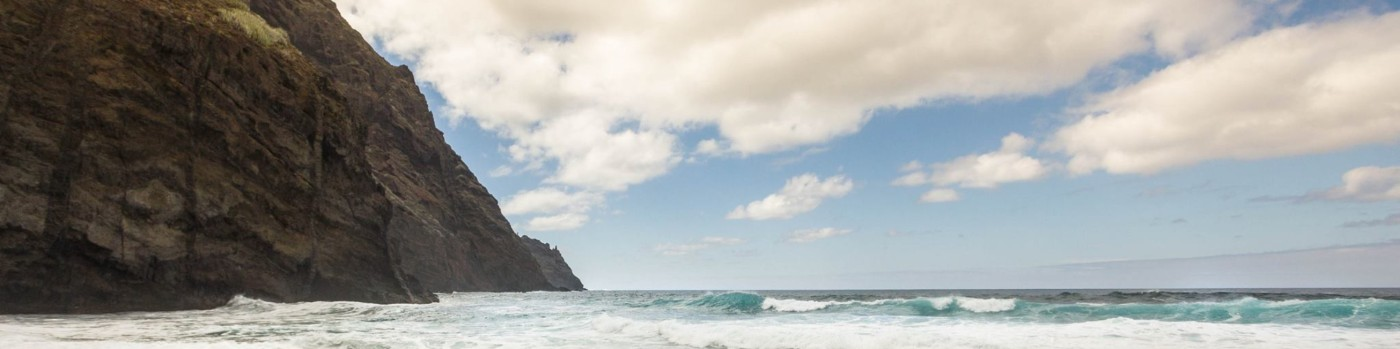
\includegraphics[width=\textwidth, keepaspectratio]{./imagenes/1692791160594.jpg}\par\vspace{1cm}
    {\LARGE \textbf{21156030: Métodos Numéricos Avanzados} \par}\par\vspace{1cm}
    {\Huge \textbf{Tarea 4}}\par\vspace{1cm}
    \vspace{13cm}
    % \vfill
    % Cuadro de color.
    \begin{tcolorbox}[colback=blue!5!white,colframe=blue!75!black]
        \centering
        {\large \textbf{Hecho por Álvaro Monforte Marín} \par}
        \vfill
        % {\normalsize \textbf{Data Scientist} \par}
        % {\normalsize \textbf{Máster Universitario en Ciencia de datos (Data Science)} \par}
    \end{tcolorbox}
    {\normalsize \textbf{11 de Septiembre de 2024} \par}
\end{titlepage}

\let\cleardoublepage\clearpage % Para que no haya páginas en blanco entre capítulos.

\setcounter{page}{1}
\pagestyle{plain}
\pagenumbering{roman}

\phantomsection
\addcontentsline{toc}{chapter}{Copyright}
\chapter*{Copyright}
\vspace{1cm}
\begin{figure}[H]
    \centering
	
\includegraphics[scale=1]{./imagenes/license.png}
\end{figure}
Esta obra está licenciada bajo la Licencia Creative Commons Atribución-NoComercial-SinDerivadas 3.0 España. 
Para ver una copia de esta licencia, visite \href{http://creativecommons.org/licenses/by-nc-nd/3.0/es/}{http://creativecommons.org/licenses/by-nc-nd/3.0/es/} 
o envíe una carta a Creative Commons, PO Box 1866, Mountain View, CA 94042, USA.

\cleardoublepage
\phantomsection % Para que el enlace nos lleve al lugar correcto.
\addcontentsline{toc}{chapter}{\'Indice general}
\tableofcontents

% listado de figuras.
\cleardoublepage
\phantomsection
\addcontentsline{toc}{chapter}{Lista de Figuras}
\listoffigures

% listado de tablas.
\cleardoublepage
\phantomsection
\addcontentsline{toc}{chapter}{Lista de Tablas}
\listoftables

% listado de abreviaturas.
\cleardoublepage
\phantomsection
% \addcontentsline{toc}{chapter}{Lista de abreviaturas}
\printglossary[title=Lista de Abreviaturas, toctitle=Lista de Abreviaturas]
% \printglossary[type=\acronymtype]

\cleardoublepage

\newpage
\setcounter{page}{1}
\pagenumbering{arabic}
\chapter{Introducción al problema}

En este informe, abordaremos la resolución de una ecuación diferencial hiperbólica con las siguientes condiciones iniciales y de frontera. Consideramos la ecuación:

\begin{equation}\label{eq:onda}
    \frac{\partial^2 u}{\partial t^2} - \frac{\partial^2 u}{\partial x^2} + (1 - x^2) = 0,
\end{equation}

definida para $x \in (0, 1)$ y $\forall t > 0$, con las siguientes condiciones de contorno y condiciones iniciales:

\begin{equation}\label{eq:condiciones}
    u(x, 0) = x(1 - x), \quad \frac{\partial u}{\partial t}(x, 0) = 0, \quad u(0, t) = 0, \quad u(1, t) = 0.
\end{equation}

La ecuación diferencial hiperbólica que nos ocupa tiene importantes aplicaciones en la física, especialmente en la modelación de ondas. En esta actividad, aplicaremos dos métodos numéricos distintos para su resolución:

\begin{itemize}
    \item El \textbf{método de diferencias finitas}, que aproximará la solución mediante discretización en el tiempo y el espacio.
    \item El \textbf{método de las características}, que es un enfoque analítico para resolver ecuaciones de onda, utilizando las curvas características de la ecuación diferencial.
\end{itemize}

Finalmente, compararemos los resultados obtenidos por ambos métodos en el mismo punto del dominio y realizaremos un análisis cuantitativo del error y de la convergencia de las soluciones numéricas.

\chapter{Metodología}

\section{Diferencias Finitas}

\section{Esquema de diferencias finitas}

El método de diferencias finitas es una técnica numérica que nos permite aproximar derivadas mediante diferencias entre valores discretos de la función. Para la ecuación diferencial dada, discretizamos tanto la coordenada espacial $x$ como el tiempo $t$.

En este caso, utilizaremos una malla uniforme de puntos $(x_i, t_n)$ con un paso espacial $\Delta x$ y un paso temporal $\Delta t$. La ecuación diferencial se puede aproximar usando diferencias centradas para las segundas derivadas espaciales y temporales:

\begin{equation}\label{eq:aprox_derivadas_centradas}
    \frac{\partial^2 u}{\partial t^2} \approx \frac{u^{n+1}_i - 2u^n_i + u^{n-1}_i}{\Delta t^2}, \quad \frac{\partial^2 u}{\partial x^2} \approx \frac{u^n_{i+1} - 2u^n_i + u^n_{i-1}}{\Delta x^2}.
\end{equation}

Sustituyendo estas aproximaciones en la ecuación diferencial, obtenemos el esquema de diferencias finitas explícito:

\begin{equation}\label{eq:dif_finitas}
    u^{n+1}_i = 2u^n_i - u^{n-1}_i + r \left( u^n_{i+1} - 2u^n_i + u^n_{i-1} \right) + \Delta t^2 (1 - x_i^2),
\end{equation}

donde $r = \left( \frac{\Delta t}{\Delta x} \right)^2$ es el coeficiente de estabilidad de \gls{cfl}, que asegura la estabilidad del esquema numérico.

Las condiciones iniciales y de frontera se aplican de la siguiente manera:

\begin{equation}\label{eq:condiciones_dif_finitas}
    u(0, t) = 0, \quad u(1, t) = 0, \quad u(x, 0) = x(1 - x), \quad \frac{\partial u}{\partial t}(x, 0) = 0.
\end{equation}

Este esquema se implementará en el código (puede verse en la subseccion \ref{implementacion_dif_finitas_python}) para obtener la solución numérica de la ecuación de onda en un dominio discreto.

\subsection{Implementación en Python para diferencias finitas}\label{implementacion_dif_finitas_python}

A continuación, se muestra la implementación en Python del esquema de diferencias finitas para resolver la ecuación de onda hiperbólica. El código se encarga de discretizar el dominio espacial y temporal, aplicar las condiciones iniciales y de frontera, y resolver la ecuación diferencial mediante un bucle temporal con criterio de convergencia.
Dentro de \texttt{main.py} (anexo \ref{apendice:b}) nos encontramos \ref{fig:codigo_dif_finitas}.


La implementación presentada utiliza el método de diferencias finitas para resolver la ecuación de onda hiperbólica en una dimensión. El dominio espacial se discretiza en $Nx$ puntos y el dominio temporal en $Nt$ pasos. A continuación, se describen los pasos clave del algoritmo:

\begin{itemize}
    \item Se definen los parámetros de discretización: $dx = L / Nx$ y $dt = T / Nt$, donde $L$ es la longitud espacial y $T$ el tiempo total de simulación. La relación de estabilidad, $\sigma = (dt/dx)^2$, es calculada y utilizada para garantizar la estabilidad del esquema.
    
    \item La matriz $u$ se inicializa para almacenar las soluciones en todos los puntos espaciales y temporales. La condición inicial para $u(x,0)$ se define como $u(x, 0) = x(1 - x)$.

    \item Se calculan los valores para el primer paso temporal ($n=1$) mediante una aproximación basada en diferencias centradas para la segunda derivada espacial, más un término fuente proporcional a $1 - x^2$.
    
    \item Se aplican condiciones de frontera de Dirichlet, donde $u(0,t) = 0$ y $u(L,t) = 0$ para todos los instantes de tiempo.
    
    \item El bucle principal recorre cada paso temporal. Para cada instante $t_n$, la solución en el siguiente instante $t_{n+1}$ se calcula utilizando un esquema explícito de diferencias finitas, basado en los valores en $t_n$ y $t_{n-1}$.

    \item Después de cada paso temporal, se verifica el criterio de convergencia calculando el cambio máximo $\Delta u = \max |u^{n+1} - u^n|$. Si el cambio máximo es menor que la tolerancia definida, el bucle se detiene indicando que la solución ha convergido.

    \item Finalmente, se devuelven los valores de $x$, el tiempo hasta el paso convergente, y la solución $u$ para todos los pasos espaciales y temporales hasta el punto de convergencia.
\end{itemize}

De esta forma, el código implementa el método de diferencias finitas para resolver la ecuación de onda con condiciones iniciales y de frontera específicas, proporcionando una aproximación numérica de la solución.

\begin{figure}[h!]
    \centering
    \begin{minted}[fontsize={\fontsize{5.5}{6.5}\selectfont}, breaklines]{python}
    
    def resolver_onda_hiperbolica(Nx: int, Nt: int, L: float, T: float, tolerancia: float = 1e-6):
        # Parámetros de discretización.
        dx = L / Nx
        dt = T / Nt
        x = np.linspace(0, L, Nx + 1)
        t = np.linspace(0, T, Nt + 1)
        sigma = (dt / dx) ** 2
    
        # Inicializar la matriz de soluciones.
        u = np.zeros((Nt + 1, Nx + 1))
    
        # Condición inicial u(x, 0) = x(1 - x).
        u[0, :] = x * (1 - x)
    
        # Condición inicial de la derivada temporal es cero.
        # Calculamos u[1, :] usando la aproximación:
        for i in range(1, Nx):
            u[1, i] = u[0, i] + 0.5 * sigma * (
                u[0, i+1] - 2*u[0, i] + u[0, i-1] + dx**2 * (1 - x[i]**2)
            )
    
        # Aplicar condiciones de frontera.
        u[:, 0] = 0  # u(0, t) = 0
        u[:, Nx] = 0  # Suponiendo u(L, t) = 0
    
        # Bucle de tiempo con criterio de convergencia.
        for n in range(1, Nt):
            u_old = u[n, :].copy()  # Copiar la solución anterior.
    
            # Actualizar solución en el paso n+1
            for i in range(1, Nx):
                u[n+1, i] = (
                    2*u[n, i] - u[n-1, i] + sigma * (
                        u[n, i+1] - 2*u[n, i] + u[n, i-1] + dx**2 * (1 - x[i]**2)
                    )
                )
    
            # Aplicar condiciones de frontera.
            u[n+1, 0] = 0
            u[n+1, Nx] = 0
    
            # Verificar criterio de convergencia.
            max_delta = np.max(np.abs(u[n+1, :] - u_old))
            if max_delta < tolerancia:
                informer.info(f'Convergencia alcanzada en el paso temporal n={n} con delta máximo={max_delta:.2e}')
                break
    
        return x, t[:n+2], u[:n+2, :]  # Devolver solo hasta el paso convergente
    
    \end{minted}
    \label{fig:codigo_dif_finitas}
    \caption{Implementación en Python del método de diferencias finitas para resolver la ecuación de onda hiperbólica.}
\end{figure}

\newpage
\section{Implementación del método de las características}
El método de las características convierte la ecuación diferencial parcial de segundo orden en un conjunto de ecuaciones diferenciales ordinarias que se resuelven a lo largo de las líneas características. Estas líneas son trayectorias en el espacio-temporal en las que las derivadas parciales de la solución se simplifican o se mantienen constantes.

Para la ecuación de onda que estamos resolviendo:

\begin{equation}
    \frac{\partial^2 u}{\partial t^2} - \frac{\partial^2 u}{\partial x^2} + (1 - x^2) = 0,
\end{equation}

las características vienen dadas por las líneas $x - t = \text{constante}$ y $x + t = \text{constante}$. Esto implica que, a lo largo de estas líneas, el comportamiento de la solución $u(x, t)$ puede estudiarse de manera simplificada. Específicamente, el método transforma la ecuación original en un conjunto de ecuaciones diferenciales ordinarias que se resuelven mediante integración a lo largo de las características.

En términos prácticos, la aplicación del método de las características consiste en los siguientes pasos:

\begin{enumerate}
    \item \textbf{Reescritura de la ecuación diferencial}: A partir de la ecuación original, se separa en dos partes a lo largo de las curvas características. Esto transforma la ecuación parcial en un conjunto de ecuaciones ordinarias que se pueden resolver con métodos convencionales.
    
    \item \textbf{Solución a lo largo de las características}: Se integran estas ecuaciones a lo largo de las líneas $x - t = \text{constante}$ y $x + t = \text{constante}$, obteniendo una solución que es válida en esas curvas específicas del espacio-tiempo.
    
    \item \textbf{Condiciones iniciales y de frontera}: El método también permite incorporar las condiciones iniciales y de frontera de la ecuación de manera directa, ya que las soluciones a lo largo de las características dependen de estos valores en los puntos de partida de las características.
    
    \item \textbf{Combinación de soluciones}: Una vez obtenidas las soluciones a lo largo de cada característica, se combinan para obtener la solución general en el dominio de interés. Esto se hace utilizando las características de la ecuación y las condiciones impuestas por el problema original.
\end{enumerate}

El método de las características es especialmente útil en este tipo de ecuaciones hiperbólicas, ya que nos permite estudiar cómo las soluciones se propagan a lo largo del tiempo y el espacio, siguiendo trayectorias bien definidas. Además, al resolver a lo largo de estas características, se evita la complejidad de tener que resolver una ecuación en dos variables directamente, reduciendo el problema a uno más manejable.

Finalmente, en la sección de resultados se comparará la solución obtenida por este método con la solución numérica basada en diferencias finitas para validar la efectividad y precisión de ambos métodos.


\chapter{Resultados y discusión}

\section{Implementación del metodo de las características}

\subsection{Paso para calcular el punto R}

\begin{itemize}
    \item \textbf{Curvas características:} Las características de una ecuación de onda hiperbólica son las líneas rectas dadas por:
    \begin{equation}
    x - t = \text{constante} \quad \text{y} \quad x + t = \text{constante}.
    \end{equation}

    \item \textbf{Puntos $P(0.2, 0)$ y $Q(0.4, 0)$:} Sabemos que las características que pasan por $P$ y $Q$ son:
    \begin{itemize}
        \item Para $P(0.2, 0)$, las curvas características son:
        \begin{equation}
        x - t = 0.2 \quad \text{y} \quad x + t = 0.2.
        \end{equation}
        
        \item Para $Q(0.4, 0)$, las curvas características son:
        \begin{equation}
        x - t = 0.4 \quad \text{y} \quad x + t = 0.4.
        \end{equation}
    \end{itemize}

    \item \textbf{Intersección en $R$:} El punto de intersección de estas dos características es el punto $R$, cuyas coordenadas $(x_R, t_R)$ deben satisfacer:
    \begin{equation}
    x - t = 0.2 \quad \text{y} \quad x + t = 0.4.
    \end{equation}

    \item Resolviendo este sistema:
    \begin{equation}\label{eq:1}
    x - t = 0.2
    \end{equation}
    \begin{equation}\label{eq:2}
    x + t = 0.4
    \end{equation}

    \item Sumando \ref{eq:1} y \ref{eq:2}:
    \begin{equation}
    2x = 0.6 \quad \Rightarrow \quad x = 0.3
    \end{equation}

    \item Restando \ref{eq:2} de \ref{eq:1}:
    \begin{equation}
    2t = 0.2 \quad \Rightarrow \quad t = 0.1
    \end{equation}
\end{itemize}

Así, el punto de intersección $R$ tiene las coordenadas $R(0.3, 0.1)$.


\section{Método de las características}

En esta sección, resolveremos la ecuación diferencial utilizando el método de las características. Consideramos las curvas características que pasan por los puntos \( P(0.2, 0) \) y \( Q(0.4, 0) \), las cuales se intersectan en el punto \( R(0.3, 0.1) \).

La ecuación diferencial es la ecuación de onda unidimensional:

\begin{equation}
\frac{\partial^2 u}{\partial t^2} - \frac{\partial^2 u}{\partial x^2} = 0
\end{equation}

La solución general de esta ecuación se puede escribir en términos de las características:

\begin{equation}
u(x,t) = f(x - t) + g(x + t)
\end{equation}

Aquí, \( f \) y \( g \) son funciones que debemos determinar usando las condiciones iniciales.

\subsection{Características}

Las curvas características para esta ecuación son líneas rectas en el plano \(x-t\) con pendientes \( \pm 1 \), es decir:

\begin{itemize}
    \item \( x - t = \text{constante} \)
    \item \( x + t = \text{constante} \)
\end{itemize}

Las características que pasan por los puntos \( P(0.2, 0) \) y \( Q(0.4, 0) \) tienen las siguientes ecuaciones:

\begin{itemize}
    \item Para el punto \(P(0.2, 0)\):
    \begin{align}
    x - t &= 0.2 \quad \text{(es decir, \(x = t + 0.2\))}, \\
    x + t &= 0.2 \quad \text{(es decir, \(x = -t + 0.2\))}.
    \end{align}

    \item Para el punto \(Q(0.4, 0)\):
    \begin{align}
    x - t &= 0.4 \quad \text{(es decir, \(x = t + 0.4\))}, \\
    x + t &= 0.4 \quad \text{(es decir, \(x = -t + 0.4\))}.
    \end{align}
\end{itemize}

El punto \( R(0.3, 0.1) \) es el punto de intersección de estas características.

\subsection{Solución en \(R(0.3, 0.1)\)}

Sabemos que la solución de la ecuación de onda está dada por:

\begin{equation}
u(x,t) = f(x - t) + g(x + t)
\end{equation}

Donde \( f \) y \( g \) son funciones que debemos determinar a partir de las condiciones iniciales:

\begin{itemize}
    \item \( u(x, 0) = x(1 - x) \)
    \item \( \frac{\partial u}{\partial t}(x, 0) = 0 \)
\end{itemize}

Primero, usemos la condición \( u(x, 0) = x(1 - x) \). Esto implica que en \( t = 0 \):

\begin{equation}
f(x) + g(x) = x(1 - x)
\end{equation}

Luego, usando la condición de velocidad inicial \( \frac{\partial u}{\partial t}(x, 0) = 0 \), tenemos que:

\begin{equation}
f'(x) - g'(x) = 0 \quad \Rightarrow \quad f'(x) = g'(x)
\end{equation}

Esto implica que \( f(x) \) y \( g(x) \) difieren solo en una constante, es decir:

\begin{equation}
f(x) = g(x) + C
\end{equation}

Sustituyendo en la ecuación \( f(x) + g(x) = x(1 - x) \), obtenemos:

\begin{equation}
g(x) + C + g(x) = x(1 - x) \quad \Rightarrow \quad 2g(x) + C = x(1 - x)
\end{equation}

Por lo tanto:

\begin{equation}
g(x) = \frac{x(1 - x) - C}{2}
\end{equation}

Y:

\begin{equation}
f(x) = \frac{x(1 - x) + C}{2}
\end{equation}

Para determinar \( C \), se necesita información adicional (por ejemplo, condiciones de frontera).

\subsection{Evaluación de \( u(0.3, 0.1) \)}

Ahora que tenemos las expresiones para \( f(x) \) y \( g(x) \), podemos evaluar \( u(0.3, 0.1) \):

\begin{equation}
u(0.3, 0.1) = f(0.3 - 0.1) + g(0.3 + 0.1) = f(0.2) + g(0.4)
\end{equation}

Sustituimos los valores de \( f(x) \) y \( g(x) \):

\begin{align}
f(0.2) &= \frac{0.2(1 - 0.2) + C}{2} = \frac{0.2 \times 0.8 + C}{2} = \frac{0.16 + C}{2}, \\
g(0.4) &= \frac{0.4(1 - 0.4) - C}{2} = \frac{0.4 \times 0.6 - C}{2} = \frac{0.24 - C}{2}.
\end{align}

Finalmente, sumamos los resultados:

\begin{equation}
u(0.3, 0.1) = \frac{0.16 + C}{2} + \frac{0.24 - C}{2} = \frac{0.16 + 0.24}{2} = \frac{0.4}{2} = 0.2
\end{equation}

\newpage
\section{Metodo de diferencias finitas}

\begin{figure}[h!]
    \centering
    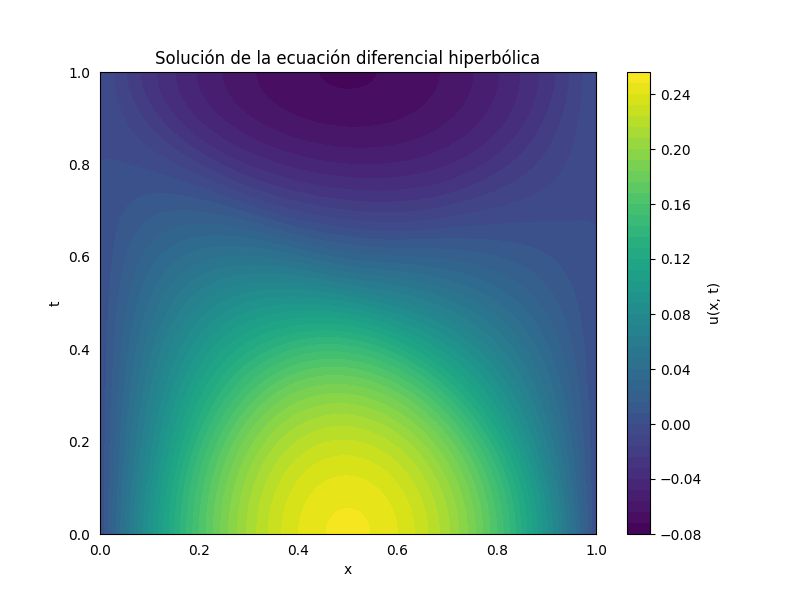
\includegraphics[width=0.8\textwidth]{figuras/ecuacion_ondas.png}
    \caption{Solución numérica de la ecuación de onda en el dominio \(x \in (0, 1)\) y \(t \in (0, 1)\).}
    \label{fig:solucion_numerica}
\end{figure}


\begin{table}[h!]
    \centering
    \begin{tabular}{lrrrr}
        \toprule
        Punto & Valor Analítico & Valor Numérico & Error Absoluto & Error Relativo \\
        \midrule
        P(0.2, 0) & 0.160000 & 0.160000 & 0.000000 & 0.000000 \\
        Q(0.4, 0) & 0.240000 & 0.240000 & 0.000000 & 0.000000 \\
        R(0.3, 0.1) & 0.200000 & 0.204542 & 0.004542 & 2.270875 \\
        \bottomrule
    \end{tabular}
    \label{tab:errores}
    \caption{Comparación de los valores analíticos y numéricos en los puntos \( P \), \( Q \) y \( R \), con errores absoluto y relativo.}        
\end{table}

\newpage
\section{Comparación de los métodos}

% Cargar la figura de la solución numérica


La figura \ref{fig:solucion_numerica} muestra la solución numérica obtenida a partir del método de diferencias finitas para la ecuación de onda hiperbólica en el dominio \(x \in (0, 1)\) y \(t \in (0, 1)\). En este método, el dominio espacial y temporal se discretiza utilizando un número de puntos \(N_x\) y \(N_t\) respectivamente, y se implementa un esquema explícito que relaciona la evolución temporal de la solución en términos de los valores presentes y pasados.

La distribución que se observa en la figura refleja la evolución de la solución \( u(x, t) \), la cual depende de las condiciones iniciales y de frontera impuestas. En particular, en esta simulación se ha supuesto que \( u(x, 0) = x(1 - x) \), lo que proporciona un perfil parabólico inicial. A medida que avanza el tiempo, este perfil evoluciona según las características de la ecuación, y la figura captura cómo la solución varía en función del tiempo y el espacio.

Además, se observa que las condiciones de frontera en \(x = 0\) y \(x = 1\) fuerzan a la solución a ser cero en estos puntos durante todo el tiempo simulado, lo que genera una simetría en el comportamiento de \(u(x,t)\) alrededor de \(x = 0.5\).


La comparación de los métodos numérico (diferencias finitas) y analítico (método de las características) es esencial para validar la precisión del método numérico. En la Tabla \ref{tab:errores}, se presenta una comparación entre los valores numéricos obtenidos en puntos específicos del dominio y los valores analíticos calculados utilizando el método de las características.

Los puntos seleccionados son \(P(0.2, 0)\), \(Q(0.4, 0)\) y \(R(0.3, 0.1)\). A continuación, se detalla la interpretación de estos resultados:

\begin{itemize}
    \item \textbf{Punto \(P(0.2, 0)\)}: El valor numérico coincide exactamente con el valor analítico, lo que sugiere que el método de diferencias finitas proporciona una excelente aproximación en este punto. El error absoluto y el error relativo son ambos cero, lo que es un buen indicativo de la precisión en los puntos iniciales.
    
    \item \textbf{Punto \(Q(0.4, 0)\)}: Similar al punto anterior, el valor numérico coincide perfectamente con el valor analítico. Esto refuerza la idea de que el método numérico reproduce de manera correcta los valores en el tiempo inicial.
    
    \item \textbf{Punto \(R(0.3, 0.1)\)}: A medida que avanzamos en el tiempo, comienzan a aparecer pequeñas discrepancias entre el valor analítico y el numérico. En este caso, el error absoluto es de 0.004542, lo cual es relativamente pequeño en términos absolutos, pero en términos relativos representa un error del 2.27%. Esta diferencia puede deberse a la acumulación de errores numéricos propios del método de diferencias finitas, que puede ser más sensible a la evolución temporal.
\end{itemize}

En general, la tabla demuestra que el método de diferencias finitas es capaz de reproducir los resultados analíticos con gran precisión en las etapas iniciales y en ciertas regiones del dominio, aunque se observa una ligera pérdida de precisión a medida que se avanza en el tiempo.

\subsection{Posibles mejoras en el método numérico}

Aunque los resultados obtenidos mediante el método de diferencias finitas son muy precisos en gran parte del dominio, hay algunas mejoras que podrían implementarse para aumentar la precisión, especialmente en puntos como \(R(0.3, 0.1)\), donde el error relativo es más significativo:

\begin{itemize}
    \item \textbf{Aumento de la resolución temporal y espacial}: Una posible solución para reducir el error es incrementar el número de puntos espaciales \(N_x\) y temporales \(N_t\), lo que llevaría a una mayor precisión en la discretización del dominio. Esto ayudaría a disminuir la acumulación de errores en la evolución temporal.

    \item \textbf{Refinamiento adaptativo de la malla}: En lugar de usar una malla uniforme, se podría emplear un método adaptativo que refine la malla en las regiones donde la solución varía más rápidamente. Esto permitiría una mejor aproximación en las zonas críticas sin aumentar innecesariamente el costo computacional en otras áreas.

    \item \textbf{Métodos de diferencias finitas de mayor orden}: El esquema utilizado es de segundo orden de precisión. Si bien esto es suficiente para muchas aplicaciones, se podría implementar un esquema de mayor orden para reducir aún más los errores numéricos.

    \item \textbf{Estudio de la estabilidad}: Aunque el método utilizado es condicionalmente estable, sería interesante estudiar más a fondo el criterio de estabilidad en función del tamaño de paso temporal y espacial para asegurarse de que no hay inestabilidades en la evolución de la solución.
\end{itemize}


Al comparar el método de diferencias finitas con el método de las características, es evidente que ambos enfoques tienen fortalezas y limitaciones. A continuación se analiza en detalle:

\begin{itemize}
    \item \textbf{Precisión del método de las características}: Este método es analíticamente exacto dentro de sus limitaciones, ya que transforma la ecuación diferencial parcial en un conjunto de ecuaciones diferenciales ordinarias que se pueden resolver de manera exacta. Sin embargo, en situaciones más complejas donde las características se cruzan o el problema involucra condiciones más complicadas, su implementación puede volverse menos práctica.

    \item \textbf{Flexibilidad del método de diferencias finitas}: Aunque el método de diferencias finitas introduce errores numéricos, es extremadamente flexible y puede manejar geometrías complejas, condiciones de frontera arbitrarias y problemas no lineales. Además, su implementación es más sencilla en problemas multidimensionales y no requiere del conocimiento exacto de las características del sistema.

    \item \textbf{Estabilidad y convergencia}: El método de diferencias finitas está sujeto a restricciones de estabilidad (por ejemplo, la relación de \gls{cfl}) y es necesario asegurar que el tamaño del paso temporal y espacial cumplen con estas condiciones para evitar inestabilidades. A diferencia del método de las características, que es inherentemente estable, el método numérico necesita ser ajustado cuidadosamente para garantizar convergencia.

    \item \textbf{Costo computacional}: El método de diferencias finitas tiende a ser más costoso computacionalmente que el método de las características, ya que requiere resolver la ecuación en una malla de puntos en el espacio y el tiempo. El método de las características, por otro lado, puede ser más eficiente, especialmente cuando el problema puede resolverse de manera analítica a lo largo de las características.

    \item \textbf{Errores y validación}: La tabla de comparación de errores muestra que el método de diferencias finitas proporciona una buena aproximación en la mayoría de los puntos estudiados, con errores absolutos y relativos muy bajos en general. Sin embargo, se observa una mayor discrepancia en puntos más alejados del tiempo inicial, lo que indica que la precisión numérica se degrada a medida que la simulación avanza.
\end{itemize}

En resumen, el método de diferencias finitas ofrece una solución numérica robusta y flexible, mientras que el método de las características proporciona una solución analítica exacta en ciertos casos específicos

% \include{ejercicios/2}
% \include{ejercicios/3}



% bibliografia
% \addcontentsline{toc}{chapter}{Bibliography}

\newpage
\clearpage
\pagestyle{plain}
\addcontentsline{toc}{chapter}{Bibliografia}
\bibliographystyle{unsrtnat}
\bibliography{referencias}

\appendix
\chapter{main.py}\label{apendice:a}

\begin{minted}[fontsize={\fontsize{5.5}{6.5}\selectfont}, breaklines]{python}

# .

# Imports necesarios
import numpy as np
import matplotlib.pyplot as plt
import pandas as pd
from pathlib import Path
import logging
import argparse

# Configuración del logger
def define_logger(logger_name='mna', logger_level='INFO'):
    logger = logging.getLogger(logger_name)
    logger.setLevel(logger_level)
    ch = logging.StreamHandler()
    ch.setLevel(logger_level)
    formatter = logging.Formatter('%(asctime)s - %(name)s - %(levelname)s - %(message)s')
    ch.setFormatter(formatter)
    logger.addHandler(ch)
    return logger

informer = define_logger(logger_name='mna', logger_level='INFO')

def resolver_laplace_polar(Nr, Ntheta, R, T0, T1, tolerancia=1e-6, max_iter=10000, omega=1.0):
    # Crear la malla
    dr = R / (Nr - 1)
    dtheta = np.pi / (Ntheta - 1)
    r = np.linspace(0, R, Nr)
    theta = np.linspace(0, np.pi, Ntheta)
    R_grid, Theta_grid = np.meshgrid(r, theta, indexing='ij')

    # Inicializar la matriz de temperaturas
    u = np.zeros((Nr, Ntheta))

    # Condiciones de frontera
    u[-1, :] = T1  # Borde circular (r = R)
    u[:, 0] = T0   # Diámetro (theta = 0)
    u[:, -1] = T0  # Diámetro (theta = pi)

    # Iteraciones
    convergencia = False
    iter_count = 0

    while not convergencia and iter_count < max_iter:
        u_old = u.copy()
        iter_count += 1

        for i in range(1, Nr - 1):
            r_i = r[i]
            if r_i == 0:
                continue  # Evitar división por cero
            beta = (r_i * dtheta / dr) ** 2
            denom = 2 * (1 + beta)
            for j in range(1, Ntheta - 1):
                u_new = (1 / denom) * (u[i+1, j] + u[i-1, j] + beta * (u[i, j+1] + u[i, j-1]))
                u[i, j] = u[i, j] + omega * (u_new - u[i, j])

        # Manejar el centro (r = 0)
        u[0, :] = np.mean(u[1, :])  # Asumir simetría radial

        # Verificar convergencia
        max_diff = np.max(np.abs(u - u_old))
        if max_diff < tolerancia:
            convergencia = True
            informer.info(f'Convergencia alcanzada en {iter_count} iteraciones con diferencia máxima {max_diff:.2e}')

    if not convergencia:
        informer.warning(f'No se alcanzó la convergencia después de {max_iter} iteraciones')

    return r, theta, u

# Función para resolver la ecuación de Laplace en coordenadas cartesianas
def resolver_laplace_cartesiano(Nx, Ny, R, T0, T1, tolerancia=1e-6, max_iter=10000, omega=1.0):
    # Crear la malla
    dx = R / (Nx - 1)
    dy = R / (Ny - 1)
    x = np.linspace(0, R, Nx)
    y = np.linspace(0, R, Ny)
    X_grid, Y_grid = np.meshgrid(x, y, indexing='ij')

    # Inicializar la matriz de temperaturas
    u = np.zeros((Nx, Ny))

    # Aplicar condiciones de frontera
    # Borde circular (x^2 + y^2 = R^2)
    for i in range(Nx):
        for j in range(Ny):
            if x[i]**2 + y[j]**2 >= R**2:
                u[i, j] = T1

    # Diámetro (y = theta)
    u[:, 0] = T0

    # Iteraciones
    convergencia = False
    iter_count = 0

    while not convergencia and iter_count < max_iter:
        u_old = u.copy()
        iter_count += 1

        for i in range(1, Nx - 1):
            for j in range(1, Ny - 1):
                # Verificar si dentro.
                if x[i]**2 + y[j]**2 < R**2 and y[j] >= 0:
                    u_new = 0.25 * (u[i+1, j] + u[i-1, j] + u[i, j+1] + u[i, j-1])
                    u[i, j] = u[i, j] + omega * (u_new - u[i, j])

        # Verificar convergencia
        max_diff = np.max(np.abs(u - u_old))
        if max_diff < tolerancia:
            convergencia = True
            informer.info(f'Convergencia alcanzada en {iter_count} iteraciones con diferencia máxima {max_diff:.2e}')

    if not convergencia:
        informer.warning(f'No se alcanzó la convergencia después de {max_iter} iteraciones')

    return x, y, u

# Función para convertir la tabla a LaTeX
def convertir_tabla_a_latex(df: pd.DataFrame, ruta_salida: str):
    latex_code = df.to_latex(index=False)
    with open(ruta_salida, 'w') as f:
        f.write(latex_code)
    informer.info(f"Tabla en formato LaTeX guardada en {ruta_salida}")

if __name__ == '__main__':
    
    # Parámetros físicos y numéricos
    parser = argparse.ArgumentParser(description='Solución de la ecuación de Laplace en una lámina semicircular.')
    parser.add_argument('--verbosity', type=str, default='INFO', help='Nivel de verbosidad del logger.')
    argumentos_parseados = parser.parse_args()
    informer.setLevel(argumentos_parseados.verbosity)

    # Rutas de salida
    TEMATICA = 'ecuacion_laplace'
    FORMATO_GRAFICAS = '.png'
    OUTPUTS = 'OUTPUTS'
    RUTA_OUTPUTS = f"./{OUTPUTS}"
    RUTA_OUTPUTS_LATEX = f"./e3_latex/figuras"
    Path(RUTA_OUTPUTS).mkdir(parents=True, exist_ok=True)
    Path(RUTA_OUTPUTS_LATEX).mkdir(parents=True, exist_ok=True)

    # Parámetros del problema
    R = 1.0  # Radio de la lámina semicircular
    T0 = 0.0  # Temperatura en el diámetro
    T1 = 50.0   # Temperatura en el borde circular

    # Parámetros numéricos para coordenadas polares
    Nr = 50  # Aumentamos la resolución para mayor precisión
    Ntheta = 50
    tolerancia = 1e-6

    # Resolver en coordenadas polares
    r_polar, theta_polar, u_polar = resolver_laplace_polar(Nr, Ntheta, R, T0, T1, tolerancia=tolerancia)

    # Obtener las temperaturas en los puntos específicos (c)
    puntos_r = [0, R/4, R/2, 3*R/4, R]
    puntos_theta = [0, np.pi/4, np.pi/2, 3*np.pi/4, np.pi]

    datos_puntos = []

    for r_val in puntos_r:
        r_idx = np.argmin(np.abs(r_polar - r_val))
        for theta_val in puntos_theta:
            theta_idx = np.argmin(np.abs(theta_polar - theta_val))
            temp = u_polar[r_idx, theta_idx]
            datos_puntos.append([f"r={r_polar[r_idx]:.2f}, theta={theta_polar[theta_idx]:.2f}", temp])

    # Crear tabla de resultados
    tabla_polar = pd.DataFrame(datos_puntos, columns=['Punto (r, theta)', 'Temperatura (°C)'])

    # Guardar la tabla en CSV y LaTeX
    tabla_polar.to_csv(f"{RUTA_OUTPUTS}/tabla_polar.csv", index=False)
    convertir_tabla_a_latex(tabla_polar, f"{RUTA_OUTPUTS}/{TEMATICA}_tabla_polar.tex")


    # Visualización de la solución numérica en coordenadas polares
    plt.figure(figsize=(8, 6))
    R_grid, Theta_grid = np.meshgrid(r_polar, theta_polar, indexing='ij')
    X = R_grid * np.cos(Theta_grid)
    Y = R_grid * np.sin(Theta_grid)
    plt.contourf(X, Y, u_polar, levels=50, cmap='hot')
    plt.colorbar(label='Temperatura (°C)')
    plt.xlabel('x')
    plt.ylabel('y')
    plt.title('Distribución de temperatura en coordenadas polares')
    plt.axis('equal')
    plt.savefig(f"{RUTA_OUTPUTS}/{TEMATICA}_polar{FORMATO_GRAFICAS}")
    plt.savefig(f"{RUTA_OUTPUTS_LATEX}/{TEMATICA}_polar{FORMATO_GRAFICAS}")

    # Parámetros numéricos para coordenadas cartesianas
    Nx = 50
    Ny = 50

    # Resolver en coordenadas cartesianas
    x_cart, y_cart, u_cart = resolver_laplace_cartesiano(Nx, Ny, R, T0, T1, tolerancia=tolerancia)

    # Obtener las temperaturas en los puntos específicos (d)
    puntos_x = [0, R/4, R/2, 3*R/4, R]
    puntos_y = [0, R/4, R/2, 3*R/4, R]

    datos_puntos_cart = []

    for x_val in puntos_x:
        x_idx = np.argmin(np.abs(x_cart - x_val))
        for y_val in puntos_y:
            y_idx = np.argmin(np.abs(y_cart - y_val))
            # Verificar si dentro.
            if x_cart[x_idx]**2 + y_cart[y_idx]**2 <= R**2 and y_cart[y_idx] >= 0:
                temp = u_cart[x_idx, y_idx]
                datos_puntos_cart.append([f"x={x_cart[x_idx]:.2f}, y={y_cart[y_idx]:.2f}", temp])

    # Crear tabla de resultados
    tabla_cartesiano = pd.DataFrame(datos_puntos_cart, columns=['Punto (x, y)', 'Temperatura (°C)'])

    # Guardar la tabla en CSV y LaTeX
    tabla_cartesiano.to_csv(f"{RUTA_OUTPUTS}/tabla_cartesiano.csv", index=False)
    convertir_tabla_a_latex(tabla_cartesiano, f"{RUTA_OUTPUTS}/{TEMATICA}_tabla_cartesiano.tex")

    # Visualización de la solución numérica en coordenadas cartesianas
    plt.figure(figsize=(8, 6))
    X_grid, Y_grid = np.meshgrid(x_cart, y_cart, indexing='ij')
    plt.contourf(X_grid, Y_grid, u_cart, levels=50, cmap='hot')
    plt.colorbar(label='Temperatura (°C)')
    plt.xlabel('x')
    plt.ylabel('y')
    plt.title('Distribución de temperatura en coordenadas cartesianas')
    plt.axis('equal')
    plt.savefig(f"{RUTA_OUTPUTS}/{TEMATICA}_cartesiano{FORMATO_GRAFICAS}")
    plt.savefig(f"{RUTA_OUTPUTS_LATEX}/{TEMATICA}_cartesiano{FORMATO_GRAFICAS}")

    informer.info("Cálculo completado y resultados guardados.")



\end{minted}
\chapter{e}\label{apendice:b}

\section{\_\_init\_\_.py}
\begin{minted}[fontsize={\fontsize{5.5}{6.5}\selectfont}, breaklines]{python}
import numpy as np
from .src.lib.matplotlib_settings import plt
import pandas as pd
\end{minted}


\section{src}

\subsection{core}

\subsubsection{\_\_init\_\_.py}
\begin{minted}[fontsize={\fontsize{5.5}{6.5}\selectfont}, breaklines]{python}

\end{minted}



\subsubsection{\_abstractas.py}
\begin{minted}[fontsize={\fontsize{5.5}{6.5}\selectfont}, breaklines]{python}
# /e/src/core/_abstractas.py

from abc import ABC, abstractmethod
from ._typing import (
    ListaStringsLike,
    DictParametrosLike
)


class Parametros(ABC):
    
    """
    # Explicacion
    Esta clase pretende facilitar el uso de guardado de parametros.
    
    ## Example
    >>> class SDEModelParameters(Parameters):
    >>>     mu = 2
    >>>     sigma = 1
    >>>     X0 = 1
    >>> 
    >>> params = SDEModelParameters()
    >>> print(params)  # Salida esperada: "Parameters: SDEModelParameters"
    >>> print(params.nombre) # Salida esperada: "SDEModelParameters"
    >>> print(params.parametros_de_la_clase())  # {'mu': 2, 'sigma': 1, 'X0': 1}
    """
    
    def __init__(self, **kwargs):
        for key, value in kwargs.items():
            setattr(self, key, value)

    def __repr__(self) -> str:
        base_class_name = self.__class__.__bases__[0].__name__
        return f"{base_class_name}: {self.__class__.__name__}"

    @property
    def nombre(self) -> str:
        return self.__repr__().split(':')[1].strip()

    @classmethod
    def lista_de_funciones_prop_de_una_clase(cls) -> ListaStringsLike:
        return [p for p in dir(cls) if isinstance(getattr(cls, p), property)]

    @classmethod
    def parametros_de_la_clase(cls) -> DictParametrosLike:
        # Obtener las propiedades de la clase
        property_names = cls.lista_de_funciones_prop_de_una_clase()
        
        # Obtener todos los atributos que no sean métodos ni propiedades internas
        internal_variables_dict = {k: v for k, v in vars(cls).items() if not k.startswith("__")}
        
        # Excluir las propiedades y los atributos internos que comienzan con "_"
        store_keys = [] + property_names
        for key in internal_variables_dict.keys():
            if key.startswith('_'): 
                store_keys.append(key)
        for key in store_keys:
            if key in internal_variables_dict:
                del internal_variables_dict[key]
        
        return internal_variables_dict
\end{minted}


\subsubsection{\_typing.py}
\begin{minted}[fontsize={\fontsize{5.5}{6.5}\selectfont}, breaklines]{python}
# /e/src/core/_typing.py

from ... import np

from typing import (
    Dict, 
    Any,
    Union,
    Tuple,
    List,
    Optional,
    TypeVar,
    Generic,
    Callable
)

__all__ = [
    'Dict', 
    'Any',
    'Union',
    'Tuple',
    'List',
    'Optional',
    'TypeVar',
    'Generic',
    'Callable',
    'HiperparametrosLike',
    'ModuloLike',
    'CoordenadaLike',
    'CoordenadasLike',
    'DictOptionsLIke',
    'InputLike',
    'ResultadosLike',
    'ListaStringsLike',
    'DictParametrosLike',
    'ListaIntLike'
]

type ResultadosLike = Dict[str, Any]
type DictOptionsLIke = Dict[str, Any]
type DictParametrosLike = Dict[str, Any]
type HiperparametrosLike = Dict[str, int | float]
type ModuloLike = float
type CoordenadaLike = float | np.ndarray | int
type CoordenadasLike = Tuple[CoordenadaLike, ...]
type InputLike = Tuple[int | float]
type ListaStringsLike = List[str]
type ListaIntLike = List[int]

\end{minted}


\subsection{lib}

\subsubsection{\_\_init\_\_.py}
\begin{minted}[fontsize={\fontsize{5.5}{6.5}\selectfont}, breaklines]{python}

\end{minted}


\subsubsection{constants.py}
\begin{minted}[fontsize={\fontsize{5.5}{6.5}\selectfont}, breaklines]{python}
# /e/src/lib/constants.py

import os
import sys
from pathlib import Path
from dataclasses import dataclass

__all__ = [
    'Rutas'
]

@dataclass(frozen=True)
class Rutas:
    RUTA_PAQUETE: str = str(Path(__file__).resolve().parents[2])
\end{minted}


\subsubsection{general.py}
\begin{minted}[fontsize={\fontsize{5.5}{6.5}\selectfont}, breaklines]{python}
# /e/lib/clases.py

from ..core._abstractas import Parametros
from ..core._typing import (
    InputsLike
)

class ParametrosProblema(Parametros):
    
    """
    Ejemplo
    ---
    >>> Temperatura.T0 = 0
    >>> Temperatura.T1 = 50
    >>> NpuntosDireccion.Nx = 100
    >>> NpuntosDireccion.Ny = 100
    >>> SemiCirculoParametros.R = 1

    >>> inputs = {
    >>>     'T0' : Temperatura.T0,
    >>>     'T1' : Temperatura.T1,
    >>>     'Nx' : NpuntosDireccion.Nx,
    >>>     'Ny' : NpuntosDireccion.Ny,
    >>>     'R' : SemiCirculoParametros.R
    >>> }

    >>> params = ParametrosProblema(dict_parametros=inputs)
    >>> params.print_parametros
    """
    
    def __init__(self, dict_parametros: InputsLike) -> None:
        self.inputs = dict_parametros
        
    def __repr__(self) -> str:
        return f"ParametrosProblema({list(self.inputs.keys())})"
        
    @property
    def print_parametros(self):
        for parametro, valor in self.inputs.items():
            print(f"{parametro:3} | {valor:6}")   
\end{minted}


\subsubsection{logger.py}
\begin{minted}[fontsize={\fontsize{5.5}{6.5}\selectfont}, breaklines]{python}
# /e/src/lib/logger.py

import logging
from logging import _nameToLevel, _levelToName
from e.src.core._typing import (
    DictParametrosLike,
)

__all__ = [
    'dict_log_level',
    'dict_level_log',
    'define_logger'
]

dict_log_level: DictParametrosLike = _nameToLevel
dict_level_log: DictParametrosLike = _levelToName

def define_logger(logger_name: str, logger_level: str = 'DEBUG'):
    
    # Configurar logger.
    logger = logging.getLogger(logger_name)
    logger.setLevel(dict_log_level[logger_level])

    console_handler = logging.StreamHandler()

    # Añadir un formato básico para los mensajes de log.
    formatter = logging.Formatter('%(name)s - %(levelname)s - %(message)s')
    console_handler.setFormatter(formatter)

    # Añadir el handler al logger.
    logger.addHandler(console_handler)
    
    return logger
\end{minted}


\subsubsection{matplotlib\_settings.py}
\begin{minted}[fontsize={\fontsize{5.5}{6.5}\selectfont}, breaklines]{python}
# /e/src/lib/matplotlib_settings.py

import matplotlib.pyplot as plt

plt.rcParams['figure.figsize'] = (9,6)
plt.rcParams['lines.linewidth'] = 3
plt.rcParams['xtick.bottom'] = False
plt.rcParams['ytick.left'] = False
pal = ["#FBB4AE","#B3CDE3", "#CCEBC5","#CFCCC4"]
\end{minted}


\subsubsection{metodos\_numericos.py}
\begin{minted}[fontsize={\fontsize{5.5}{6.5}\selectfont}, breaklines]{python}
# /e/src/lib/metodos_numericos.py

from ... import np
from .logger import define_logger
from ..core._typing import Callable

__all__ = [
    'solve_wave_eq',
    'jacobi',
    'gauss_seidel',
    'gauss_seidel_sor'
]

informer = define_logger(logger_name='mna', logger_level='INFO')

def DiferenciasFinitas2D(
    u: np.ndarray, 
    Nx: int, 
    Ny: int, 
    update_rule: Callable[[np.ndarray, int, int], float],  # Función para actualizar u[i,j]
    tol: float = 1e-6,
    max_iter: int = int(1e4)
    ) -> np.ndarray:
    
    for iteracion in range(max_iter):
        u_old = np.copy(u)
        
        # Iterar sobre los puntos internos.
        for i in range(1, Nx-1):
            for j in range(1, Ny-1):
                # Llamada a la regla de actualización que depende de la ecuación.
                u[i, j] = update_rule(u_old, i, j)
        
        # Criterio de convergencia
        error = np.max(np.abs(u - u_old))
        if error < tol: 
            print(f"Convergencia alcanzada después de {iteracion} iteraciones.")
            return u, iteracion
        
    print(f"No se alcanzó la convergencia después de {max_iter} iteraciones.")
    return u, max_iter

def solve_wave_eq(Nx, Nt, L, T, cfl):
    """
    Resuelve la ecuación de onda hiperbólica con el esquema explícito en diferencias finitas.
    
    Args:
    - Nx: Número de puntos en la dirección espacial (x).
    - Nt: Número de puntos en la dirección temporal (t).
    - L: Longitud del dominio espacial.
    - T: Tiempo total a simular.
    - cfl: Número de Courant (CFL), define la relación entre dt y dx.
    
    Returns:
    - u: Matriz con las soluciones aproximadas.
    - x: Vector de posiciones espaciales.
    - t: Vector de tiempos.
    """
    # Discretización espacial y temporal
    dx = L / (Nx - 1)
    dt = cfl * dx  # Para mantener la estabilidad, dt <= dx/c
    x = np.linspace(0, L, Nx)
    t = np.linspace(0, T, Nt)
    
    # Coeficiente de estabilidad CFL
    r = (dt / dx)**2
    
    # Inicialización de la solución
    u = np.zeros((Nt, Nx))
    informer.debug(u)
    
    # Condiciones iniciales
    u[0, :] = x * (1 - x)  # u(x, 0) = x(1 - x)
    
    # Primera iteración: derivada temporal cero
    u[1, :] = u[0, :]  # u_t(x, 0) = 0 implica que u[1, :] = u[0, :]
    
    # Aplicar condiciones de frontera
    u[:, 0] = 0  # u(0, t) = 0
    u[:, -1] = 0  # u(1, t) = 0
    
    # Iteraciones en el tiempo
    for n in range(1, Nt-1):
        for i in range(1, Nx-1):
            u[n+1, i] = (2 * u[n, i] - u[n-1, i] +
                         r * (u[n, i+1] - 2 * u[n, i] + u[n, i-1]) +
                         dt**2 * (1 - x[i]**2))
    
    return u, x, t


def solve_wave_eq(Nx, Nt, L, T, cfl):
    """
    Resuelve la ecuación de onda hiperbólica con el esquema explícito en diferencias finitas.
    
    Args:
    - Nx: Número de puntos en la dirección espacial (x).
    - Nt: Número de puntos en la dirección temporal (t).
    - L: Longitud del dominio espacial.
    - T: Tiempo total a simular.
    - cfl: Número de Courant (CFL), define la relación entre dt y dx.
    
    Returns:
    - u: Matriz con las soluciones aproximadas.
    - x: Vector de posiciones espaciales.
    - t: Vector de tiempos.
    """
    # Discretización espacial y temporal
    dx = L / (Nx - 1)
    dt = cfl * dx  # Para mantener la estabilidad, dt <= dx/c
    x = np.linspace(0, L, Nx)
    t = np.linspace(0, T, Nt)
    
    # Coeficiente de estabilidad CFL
    r = (dt / dx)**2
    
    # Inicialización de la solución
    u = np.zeros((Nt, Nx))
    informer.debug(u)
    
    # Condiciones iniciales
    u[0, :] = x * (1 - x)  # u(x, 0) = x(1 - x)
    
    # Primera iteración: derivada temporal cero
    u[1, :] = u[0, :]  # u_t(x, 0) = 0 implica que u[1, :] = u[0, :]
    
    # Aplicar condiciones de frontera
    u[:, 0] = 0  # u(0, t) = 0
    u[:, -1] = 0  # u(1, t) = 0
    
    # Iteraciones en el tiempo
    for n in range(1, Nt-1):
        for i in range(1, Nx-1):
            u[n+1, i] = (2 * u[n, i] - u[n-1, i] +
                         r * (u[n, i+1] - 2 * u[n, i] + u[n, i-1]) +
                         dt**2 * (1 - x[i]**2))
    
    return u, x, t

def jacobi(u, Nx, Ny, tol=1e-6, max_iter=10000):
    
    for iteracion in range(max_iter):
        u_old = np.copy(u)
        
        # Iterar sobre los puntos internos.
        for i in range(1, Nx-1):
            for j in range(1, Ny-1):
                # Esquema para la ecuacion de Laplace.
                u[i, j] = 0.25 * (u[i+1, j] + u[i-1, j] + u[i, j+1] + u[i, j-1])
        
        # Criterio de convergencia
        error = np.max(np.abs(u - u_old))
        if error < tol:
            informer.info(f"Convergencia alcanzada después de {iteracion} iteraciones.")
            return u, iteracion
        
    informer.info(f"No se alcanzó la convergencia después de {max_iter} iteraciones.")
    return u, max_iter


def gauss_seidel(u, Nx, Ny, tol=1e-6, max_iter=10000):
    """
    Método de Gauss-Seidel para resolver el sistema de ecuaciones discretizado
    de la ecuación de Laplace.
    
    Args:
    - u: Matriz con las condiciones iniciales de temperatura.
    - Nx: Número de puntos en la dirección x.
    - Ny: Número de puntos en la dirección y.
    - tol: Tolerancia para la convergencia.
    - max_iter: Máximo número de iteraciones.
    
    Returns:
    - u: Matriz con las soluciones aproximadas.
    - iteraciones: Número de iteraciones realizadas.
    """
    for iteracion in range(max_iter):
        max_error = 0.0
        
        # Iterar sobre los puntos internos
        for i in range(1, Nx-1):
            for j in range(1, Ny-1):
                # Guardar el valor anterior
                u_old = u[i, j]
                
                # Esquema para la ecuación de Laplace
                u[i, j] = 0.25 * (u[i+1, j] + u[i-1, j] + u[i, j+1] + u[i, j-1])
                
                # Calcular el error máximo
                max_error = max(max_error, abs(u[i, j] - u_old))
        
        
        # Criterio de convergencia
        if max_error < tol:
            informer.info(f"Convergencia alcanzada después de {iteracion} iteraciones.")
            return u, iteracion
        
    informer.info(f"No se alcanzó la convergencia después de {max_iter} iteraciones.")
    return u, max_iter


def gauss_seidel_matriz(A, b, tol=1e-6, max_iter=10000):
    """
    Método de Gauss-Seidel para resolver un sistema lineal Ax = b.
    
    Args:
    - A: Matriz de coeficientes.
    - b: Vector de términos independientes.
    - tol: Tolerancia para la convergencia.
    - max_iter: Máximo número de iteraciones.
    
    Returns:
    - x: Vector solución.
    - iteraciones: Número de iteraciones realizadas.
    """
    n = len(b)
    x = np.zeros_like(b, dtype=np.double)  # Vector inicial de solución
    
    for iteracion in range(max_iter):
        x_old = np.copy(x)
        
        # Iterar sobre cada ecuación del sistema
        for i in range(n):
            sigma = 0
            for j in range(n):
                if i != j:
                    sigma += A[i, j] * x[j]
            
            # Actualizar la solución usando los valores más recientes
            x[i] = (b[i] - sigma) / A[i, i]
        
        # Criterio de convergencia
        error = np.linalg.norm(x - x_old, ord=np.inf)
        if error < tol:
            informer.info(f"Convergencia alcanzada después de {iteracion} iteraciones.")
            return x, iteracion
    
    informer.info(f"No se alcanzó la convergencia después de {max_iter} iteraciones.")
    return x, max_iter


def gauss_seidel_sor(u, Nx, Ny, omega=1.5, tol=1e-6, max_iter=10000):
    
    for iteracion in range(max_iter):
        max_error = 0.0
        
        # Iterar sobre los puntos internos
        for i in range(1, Nx-1):
            for j in range(1, Ny-1):
                # Guardar el valor anterior
                u_old = u[i, j]
                
                # Esquema para la ecuación de Laplace (Gauss-Seidel + Sobrerrelajación)
                u_new = 0.25 * (u[i+1, j] + u[i-1, j] + u[i, j+1] + u[i, j-1])
                
                # Actualización con Sobrerrelajación
                u[i, j] = (1 - omega) * u_old + omega * u_new
                
                # Calcular el error máximo
                max_error = max(max_error, abs(u[i, j] - u_old))
        
        # Criterio de convergencia
        if max_error < tol:
            informer.info(f"Convergencia alcanzada después de {iteracion} iteraciones.")
            return u, iteracion
    
    informer.info(f"No se alcanzó la convergencia después de {max_iter} iteraciones.")
    return u, max_iter
\end{minted}


\subsubsection{parsers.py}
\begin{minted}[fontsize={\fontsize{5.5}{6.5}\selectfont}, breaklines]{python}
# /e/src/lib/parsers.py

import argparse
from .logger import (
    dict_log_level,
    dict_level_log
)
from ..core._typing import Any

def define_parser(mensaje_descripcion: str = "Este script procesa datos para MNA.") -> Any:

    parser = argparse.ArgumentParser(description=mensaje_descripcion)

    parser.add_argument(
        "-vsy", "--verbosity",
        type=int,
        choices=[level for level in dict_log_level.values()],
        default='INFO',
        help=f"Nivel de verbosidad {list(dict_log_level.items())}"
    )

    parser.add_argument(
        "-sp", "--show_plots", 
        action="store_true",
        help="Muestra los plots del script."
    )

    parser.add_argument(
        "-pl", "--parallel", 
        action="store_true",
        help="Hace los calculos (los que procedan) en paralelo."
    )
    
    return parser
\end{minted}


\subsubsection{placeholders.py}
\begin{minted}[fontsize={\fontsize{5.5}{6.5}\selectfont}, breaklines]{python}
# /e/src/lib/placeholders.py

from ..core._typing import Optional
from ..core._abstractas import Parametros

__all__ = [
    'ParametrosFisicos',
    'NpuntosDireccion',
    'ParametrosGeometricos',
    'ParametrosComputacionales'
]

class ParametrosFisicos(Parametros):
    pass

class NpuntosDireccion(Parametros):
    pass

class ParametrosGeometricos(Parametros):
    pass

class ParametrosComputacionales(Parametros):
    pass
\end{minted}


% \include{anexo/apendiceB}

\end{document}

%%%%%%%%%%%%%%%%%%%%%%%%%%%%%%%%%%%%